\RequirePackage{luatex85}
\documentclass[tikz]{standalone}
% Default preamble
\usepackage{pgfplots}
\pgfplotsset{compat=newest}
\usepgfplotslibrary{groupplots}
\usepgfplotslibrary{polar}
\usepgfplotslibrary{smithchart}
\usepgfplotslibrary{statistics}
\usepgfplotslibrary{dateplot}
\usepgfplotslibrary{ternary}
% Custom preamble from global variable:
\usetikzlibrary{patterns}
\usepackage{xcolor}
\definecolor{cred}{HTML}{ED1C24}
\definecolor{cgrey}{HTML}{7F7F7F}
\definecolor{cblue}{HTML}{00A2E8}
\definecolor{cgreen}{HTML}{22B14C}
\definecolor{cyellow}{HTML}{FFF200}
\definecolor{corange}{HTML}{EA7904}
\definecolor{cpurple}{HTML}{9100FC}
\definecolor{julia1}{HTML}{1F77B4}
\definecolor{julia2}{HTML}{FF7F0E}
\definecolor{julia3}{HTML}{2CA02C}
\definecolor{julia4}{HTML}{D62728}
\begin{document}
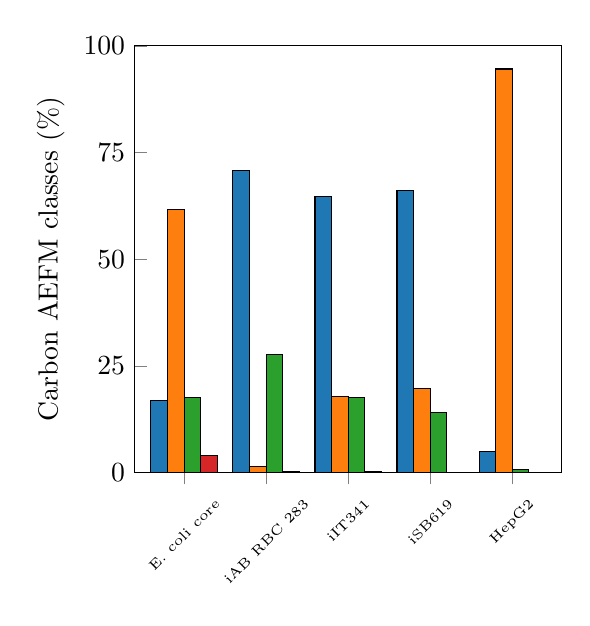
\begin{tikzpicture}
\begin{axis}[height={7cm}, width={7cm}, ybar = 0pt, xmajorgrids={false}, ymajorgrids={false}, xtick pos = bottom, ytick pos = left, bar width = 6pt, enlarge x limits = 0.15, enlarge y limits = false, legend image code/.code={\draw [#1] (0cm,-0.1cm) rectangle (0.2cm,0.25cm); }, legend style={legend columns={2}, font=\tiny}, ymax={100}, ymin={0}, xmax={5}, xtick={1,2,3,4,5}, xticklabels={E. coli core,iAB RBC 283,iIT341,iSB619,HepG2}, xticklabel style = {font=\tiny, align=center,rotate=45}, ytick={0,25,50,75,100}, ylabel={Carbon AEFM classes (\%)}]
    \addplot[black, fill=julia1]
        coordinates {
            (1,16.79705476300046)
            (2,70.74641869816537)
            (3,64.61985440537981)
            (4,66.1664760110356)
            (5,4.817056222454292)
        }
        ;
    \addplot[black, fill=julia2]
        coordinates {
            (1,61.573861021629085)
            (2,1.331992963056044)
            (3,17.732510691084777)
            (4,19.675661126438328)
            (5,94.56020122835804)
        }
        ;
    \addplot[black, fill=julia3]
        coordinates {
            (1,17.625402669121033)
            (2,27.64513696908771)
            (3,17.530114582313193)
            (4,14.127582262297288)
            (5,0.6077926639606891)
        }
        ;
    \addplot[black, fill=julia4]
        coordinates {
            (1,4.003681546249425)
            (2,0.2764513696908771)
            (3,0.11752032122221134)
            (4,0.030280600228786758)
            (5,0.014949885226973368)
        }
        ;
\end{axis}
\end{tikzpicture}
\end{document}
